\documentclass[11pt]{article}

\usepackage[T2A]{fontenc}
\usepackage[utf8]{inputenc}
\usepackage[russian]{babel}

\usepackage{indentfirst}
\usepackage{geometry}

\usepackage{amsmath, amssymb, amsfonts, amsthm, amscd}
\usepackage{mathrsfs}

\usepackage{caption}
\usepackage{graphicx}
\usepackage[all]{xy}

\geometry{a4paper}
\sloppy


\theoremstyle{plain}
\newtheorem{statement}{Утверждение}
\theoremstyle{definition}
\newtheorem{definition}{Определение}
\newtheorem*{corollary}{Следствие}
\theoremstyle{remark}
\newtheorem*{remark}{Замечание}

\renewcommand{\le}{\leqslant}
\renewcommand{\ge}{\geqslant}
\renewcommand{\phi}{\varphi}
\renewcommand{\epsilon}{\varepsilon}
\renewcommand{\kappa}{\varkappa}

\newcommand{\comdots}{,\!..}

\DeclareMathOperator*{\Hom}{Hom}
\DeclareMathOperator*{\Tor}{Tor}
\DeclareMathOperator*{\Obj}{Obj}
\DeclareMathOperator*{\Arr}{Arr}
\DeclareMathOperator*{\Fund}{Fund}
\DeclareMathOperator*{\codom}{codom}
\DeclareMathOperator*{\id}{id}
\DeclareMathOperator*{\subdim}{\lfloor \dim \rfloor}

\renewcommand{\thesubsubsection}{\roman{subsubsection}.}

\begin{document}

\author{А.~A.~Владимиров}
\title{Характер группоида}
\date{16.06.2022}
\maketitle

\section*{Задача}

    Дан функтор $\kappa = (\kappa_1, \kappa_2): \mathbf{Cat}(\Gamma) \to 
    \mathbf{Vec}$.\\
    Найти $\kappa_2 : (f: \Gamma_1 \to \Gamma_2) \mapsto 
    (A_f: \kappa_1(\Gamma_1) \to \kappa_1(\Gamma_2))$, если известно, что 
    $\kappa_1 : \Gamma \mapsto V$, где $V$ -- пространство характеров, т.е. 
    $V = \{\chi: \Hom \Gamma \to \mathbb{C}: \chi(\psi \circ \phi) = 
    \chi(\psi) + \chi(\phi)\}$.

    Таким образом задача сводится к нахождению линейного оператора $A_f$ на 
    коммутативной диаграмме 

    \begin{figure}[h]
        \centering
        \[\xymatrix{
            \Gamma_1 \ar[dd]^{\textstyle{f}} \ar[rr]^{\textstyle{\kappa}} & & V_1 \ar[dd]^{\textstyle{A_f}} \\
                                            & & \\
            \Gamma_2 \ar[rr]^{\textstyle{\kappa}}           & & V_2
        }\]
        \caption{постановка задачи}
        \label{cd_problem}
    \end{figure}

\section*{Решение}
\tableofcontents

\subsection{Характер группоида}
            \subsubsection{Группоид}
    Обсудим сперва структуру группоида общего вида\footnote{здесь и далее под 
    группоидами подразумеваются связные группоиды}
    \begin{definition}\cite{MacLane}
        \emph{Группоидом} назывется категория, в которой любая стрелка обратима.
    \end{definition}

    Для этого введем операцию произведения множеств стрелок, корректную тогда и 
    только тогда, когда все упорядоченные пары стрелок взятые из 
    соответствующих множеств перемножаемы, итак
    \begin{equation}\label{cdot_def}
        A \cdot B \doteqdot \{f\circ g \:|\: \forall f \in A, \forall g \in B\},
    \end{equation}
    в частности, если $A$ --- одноэлементное множество, имеем
    \[f \cdot B \doteqdot \{f\circ h \:|\: \forall g \in B\}.\]

    Теперь упомянем пару утверждений, справдливых для любого группоида.

    \bigskip

    Общеизвестно, что в группоиде все группы петель изоморфны, иначе говоря 
    верно
    \begin{statement}\label{st_loop_iso}
        Для любых $a$, $b$ $\in \Obj(\Gamma)$
        \begin{equation}
            \hom(b,b) = h\hom(a,a)h^{-1},
        \end{equation}
        где $h$ --- произвольная стрелка из $a$ в $b$.
    \end{statement}

    \bigskip

    Также имеет место
    \begin{statement}\label{st_gr_shift}
        Для любых различных вершин $a$, $b$ $\in \Obj(\Gamma)$ справедливо
        \begin{equation}\label{eq_fhom}
            \hom(a,b) = f \cdot \hom(a,a),
        \end{equation}
        где $f$ --- произвольная стрелка из $a$ в $b$.
    \end{statement}
    \begin{proof}
        Вложение правого множества в левое справедливо в силу аксиом 
        композиции в категории.
    
        Обратное вложение имеет место, так как для любого $g \in \hom(a,b)$ 
        найдется $h \in \hom(a,a)$ такое, что $g = fh$, а именно $h = f^{-1}h$.
    \end{proof}

    \begin{corollary}
        Пользуясь утверждениями \ref{st_loop_iso}, \ref{st_gr_shift} или 
        непосредственно, несложно доказать, что:
        \begin{gather*}
            \hom(a,b) = \hom(b,b) \cdot f,\quad f:a\to b\\
            \hom(a,b) \cdot \hom(a,a) = \hom(b,b) \cdot \hom(a,b) = \hom(a,b),\\
            \hom(b,c) \cdot \hom(a,b) = \hom(a,c). 
        \end{gather*}
    \end{corollary}

    \bigskip

    Утверждения \ref{st_loop_iso}, \ref{st_gr_shift} и их следствия позволяют 
    заключить, что по заданному группоиду можно построить категорию, с тем же 
    набором вершин и стрелками вида $\hom(a,b) : a \to b$, которая также 
    является группоидом, иначе говоря можно ввести следующее

    \begin{definition}
        Пусть $G = \Fund \Gamma$ --- фундаментальная группа группоида. 
        \emph{Фактор-группоидом} или \emph{факторизацией группоида $\Gamma$ по 
        фундаментальной группе}\footnote{в действительности можно вводить 
        факторизацию группоида по любой нормальной подгруппе фунадментальной 
        группы} 
        называется группоид $\Gamma/G$ такой, что 
        \begin{gather*}
            \Obj \Gamma/G = \Obj \Gamma,\\
            \Arr \Gamma/G = \{\hom(a,b) : a \to b \:|\: \forall a,b \in \Obj (\Gamma)\}.
        \end{gather*}
    \end{definition}

    Подобно каноническому гомоморфизму отоброжающему группу в фактор-группу, 
    можно опрделить \emph{канонический функтор} $\epsilon$ переводящий $\Gamma$ 
    в $\Gamma/G$, а именно $\epsilon : a \mapsto a$, 
    $\epsilon : (f: a \to b) \mapsto (\hom(a,b) = \epsilon(f) : a \to b)$.
    
    \bigskip

    Удобнее однако, зафиксировать некоторую вершину $a$ группоида $\Gamma$, ее 
    группу петель $\hom(a,a) = A$, и \emph{веер стрелок}
    \footnote{\textbf{Определение.} \emph{Веером стрелок} вершины 
    $a$ группоида $\Gamma$ называется множество состоящее из стрелок исходящих 
    из вершины $a$ по одной в каждую из прочих.}
     $f,g,\ldots$ Тогда, в силу утверждений \ref{st_loop_iso}, 
    \ref{st_gr_shift} стрелки группоида $\Gamma /G$ имеют вид $fA$, $fAf^{-1}$, 
    $gA,\ldots$, и отображение, осуществляемое функтором $\epsilon$ приобретает 
    вид:

    \begin{figure}[h]
        \centering
        \[\xymatrix{
            b \ar@(u,l)[]_{\textstyle{\id_b}}\ar@{-->}[ddrr]^{\textstyle{h=g \circ f^{-1}}}     & &   &                                                     & b \ar@(u,l)[]_{\textstyle{fAf^{-1}}} \ar@{-->}[ddrr]^{\textstyle{g A f^{-1}}}     & &  \\
                                                                                                & &   & \stackrel{\textstyle{\epsilon}}{\longrightarrow}    &                                                                                   & &  \\
            a \ar@(l,d)[]_{\textstyle{\id_a}} \ar[uu]^{\textstyle{f}} \ar[rr]_{\textstyle{g}}   & & c &                                                     & a \ar@(l,d)[]_{\textstyle{A}} \ar[uu]^{\textstyle{fA}} \ar[rr]_{\textstyle{gA}}   & & c
        }\]
        \caption{канонический функтор}
        \label{cd_can_func}
    \end{figure}

    Пусть читателя не смущает произвол в выборе вершины $a$ и веера стрелок, ибо 
    вне зависимости от него стрелки вида $fA : a \to b$ все равны $\hom(a,b)$ как множества. 
    Преимущество такой записи состоит в ее наглядности и удобстве полученной 
    "<алгебры"> операций в фактор-группоиде. Выведем эти операции, пользуясь 
    утверждениями 
    \ref{st_loop_iso},\ref{st_gr_shift}, их следствиями и введенной операцией
    \ref{cdot_def} перемножения множеств стрелок:

    \emph{обращение стрелки} $fA : a \to b$ :
    \[(fA)^{-1} =  f^{-1} \hom(b,b) = f^{-1} fAf^{-1} = Af^{-1} : b \to a;\]

    \emph{композиция стрелок} $Ah : b \to a$ и $gA : a \to c$ :
    \[gA \cdot Ah = gAh : b \to c.\]

    Так, ясно, как получена стрелка $gAf^{-1}$ на рис.~\ref{cd_can_func}:
    \[gA \cdot (fA)^{-1} = gA \cdot Af^{-1} = gAf^{-1}.\]

    Заметим, что в полученном группоиде $\epsilon(\Gamma)$ любая стрелка 
    $a \to b$ представлена в единственном экземпляре (и равна $\hom(a,b)$), 
    группоиды подобного вида назовем \emph{элементарными}.

\newpage    \subsubsection{Элементарный группоид}

\begin{definition}
    \emph{Элементарным группоидом} будем называть группоид для любых двух 
    вершин $a$ и $b$ которого существует одна и притом только одна стрелка 
    $f: a \to b$.
\end{definition}

\begin{figure}[h]
    \centering
    \[\xymatrix{
        b \ar@{-->}[ddrr]^{\textstyle{h=g \circ f^{-1}}}                                    & &     \\
                                                                                            & &     \\
        a \ar@(l,d)[]_{\textstyle{\id_a}} \ar[uu]^{\textstyle{f}} \ar[rr]_{\textstyle{g}}   & & c
    }\]
    \caption{элементарный группоид}
    \label{cd_el_func}
\end{figure}

Такие группоиды представляют для нас интерес ввиду простоты своей структуры. 
Более того, такие группоиды можно свести всего навсего к вееру стрелок.

\begin{statement}\label{st_veer}
    Элементарный группоид $E$ однозначно задается любым веером своих стрелок.\\
    Более строго: пусть задан дан веер стрелок $V = \{f : a \to b, g : a \to c. \ldots\}$ 
    вершины $a$ некоторого элементарного группоида $E$. Минимальный по 
    включению группоид, содержащий данный веер есть сам $E$.
\end{statement}

\begin{proof}
    Пусть $\Gamma$ --- Минимальный по включению группоид, содержащий $V$, тогда из 
    определения веера (стрелки проведены из $a$ в каждую из прочих вершин $E$) 
    получаем что $\Obj E \subset \Obj \Gamma$.

    Пользуясь аксиомами композции в категории из стрелок в $V$ можно получить 
    стрелку между любыми двумя вершинами в из $\Obj E$, т.е. по определению 
    элементарного группоида все $\Arr E$. Таким образом, $\Arr E \subset 
    \Arr \Gamma$, а поскольу $\Gamma$ --- минимальный, то $\Gamma = E$.
\end{proof}
\newpage    \subsubsection{Снова группоид}
    Вернемся к группоиду общего вида и попытаемся задать характер на нем.

    Пусть характер $\chi$ задан на фундаментальной группе группоида $\Gamma$. 
    Для определенности пусть задано $\chi : A \to \mathbb{C}$, 
    где $A = \hom(a,a), a \in \Obj \Gamma$.

    \begin{itemize}
        \item перейти к фактор группоиду;
        \item породить фактор группоид веером;
        \item отсюда характер на любом $\hom(b,c)$ задан через $f^{-1}$,$g$ и $A$;
        \item задаем характер на фактор группоиде через характер на элементарном группоиде натянутом на веер $f$,$g$,\dots;
        \item получаем (при данном характере на $A$) характер на всем группоиде;
        \item осталось понять как задать характер на $A$!
    \end{itemize}
    
\newpage    \subsubsection{Группа}
    Рассмотрим некоторую группу $G$, ее фактор-группу $G/G'$ по коммутанту 
    $G'$ и следующую диаграмму

    \begin{figure}[h]
        \centering
        \[\xymatrix{
            G \ar[rr]^{\textstyle{\tau}} \ar[rrdd]_{\textstyle{\chi}} & & G/G'\ar[dd]^{\textstyle{\chi_{ab}}} \\
            & & \\
            & & \mathbb{C}
        }\]
        \caption{}
        \label{cd_ab}
    \end{figure}

    Здесь $\tau: g \mapsto gG'$ --- канонический гомоморфизм; $\chi$, 
    $\chi_{ab}$ --- характеры групп $G$ и $G/G'$ соответственно.

    Оказывается, что 

    \begin{lemma}\label{lm_const} Для любых $f, g \in G$, таких что $f = g \mod G'$:
        \[\chi(f) = \chi(g).\]
    \end{lemma}

    \begin{proof} Действительно, в условиях леммы существует $h \in G'$, 
        такой что $f = gh$, но по определению коммутанта существуют такие 
        $a$ и $b \in G'$, что \\$h = aba^{-1}b^{-1}$, откуда $f = gaba^{-1}b^{-1}$, и 
        \[\chi(f) = \chi(gaba^{-1}b^{-1}) 
        = \chi(g) + \chi(a) + \chi(b) - \chi(a) - \chi(b) = \chi(g).\]
    \end{proof}

    Иными словами доказано, что факторизация 
    группы по коммутанту $G'$ разбивает ее на области постоянства
    характера (рис. \ref{img_chi_factor}). А значит вместо 
    рассмотрения характера $\chi$ на всей группе, достаточно пронаблюдать 
    лишь за его "<действием с точностью до $G'$">, т.е. за некоторым характером
    $\chi_{ab}$ на $G/G'$.

    \begin{figure}[h]
        \centering
        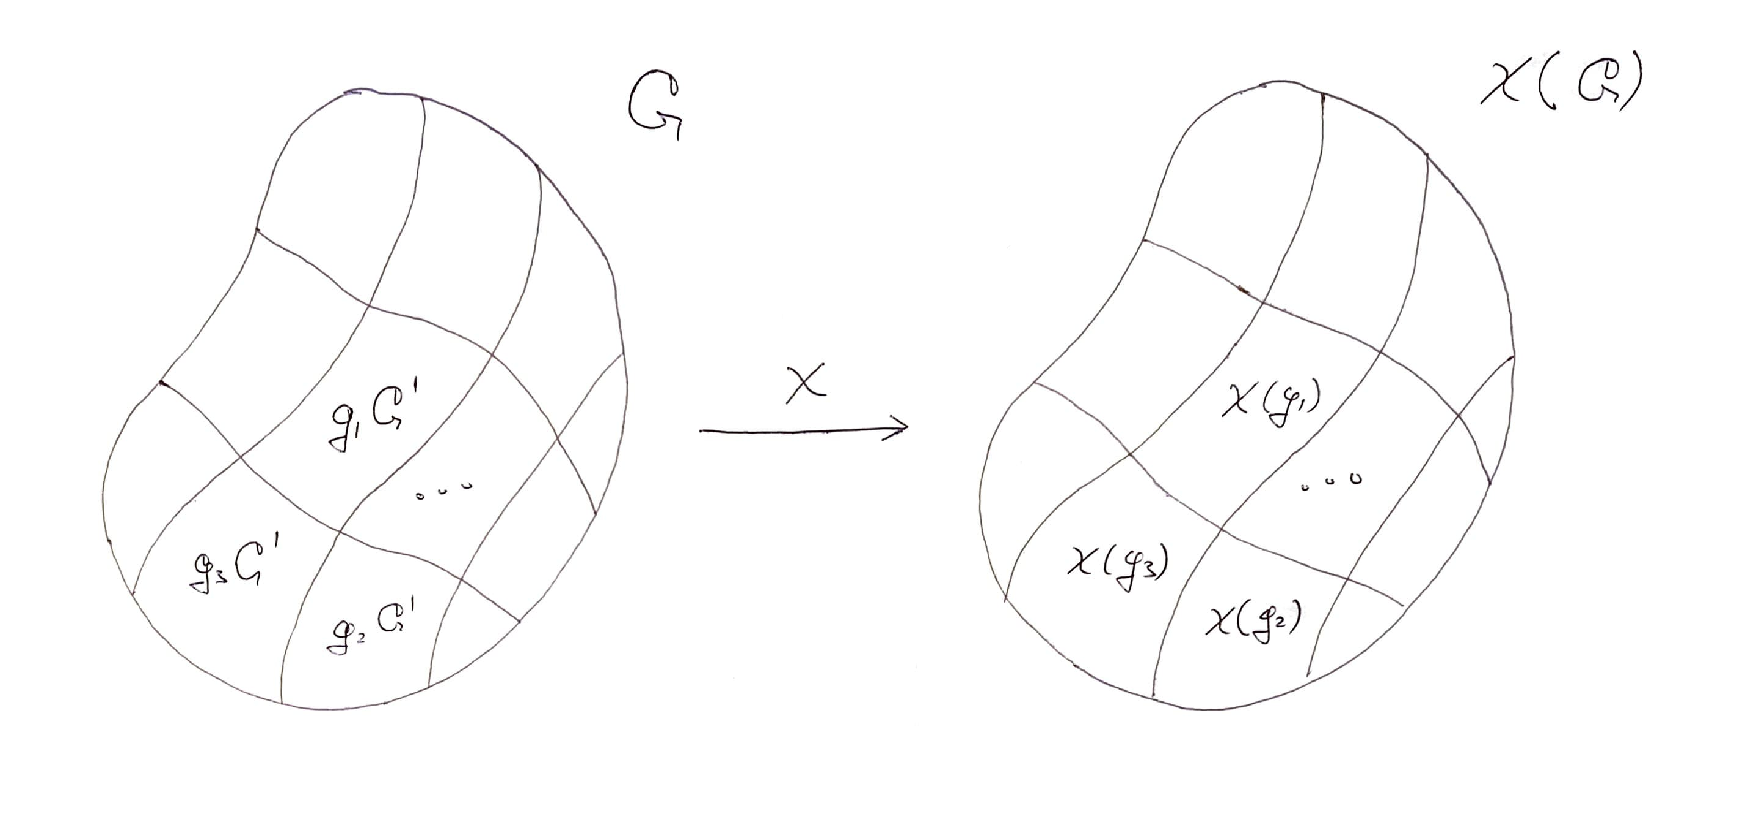
\includegraphics[width=\textwidth]{pictures/chips}
        \caption{}
        \label{img_chi_factor}
    \end{figure}

    Так, введем, очевидно инъективный, гомоморфизм 
    $t: X(G/G') \to X(G)$ пространств характеров:
    \begin{equation}
        t : \chi_{ab} \mapsto \chi_{ab} \circ \tau = \chi. 
    \end{equation}
    Его сюръективность вытекает напрямую из леммы \ref{lm_const}, ибо для 
    любого $\chi : G \to \mathbb{C}$ корректно задан $\chi_{ab}$:
    \[\chi_{ab}(gG') = \chi(g),\]
    который удовлетворяет 
    \[\chi_{ab} \circ \tau = \chi.\]
    Тем самым доказано
    \begin{statement}\label{st_char_gr_to_ab}
        \[X(G) \simeq X(G/G')\]
    \end{statement}
    Позволяющее свести характер группы к характеру ее абелизации, что и 
    приводит нас к следующему параграфу.
    
\newpage    \subsubsection{Абелева группа}
    Итак, пусть некоторая группа $A$ --- абелева. Известно, что для 
    \emph{конечно-порожденных} абелевых групп справедливо разложение 
    (\cite{Vinberg} гл.9 \S 1)
    \begin{equation*}\label{A_decomp}
        A = \sub{A} \oplus \Tor A,
    \end{equation*}
    где $\sub{A} \simeq \mathbb{Z}^{n}$ --- \emph{свободная подгруппа},\\ 
    $\Tor A \doteqdot \{a \in A: ma = 0\text{ для некоторого }m \in 
    \mathbb{Z}, m \ne 0\}$ --- \emph{подгруппа кручения}, причем
    \begin{equation*}\label{TorA_decomp}
        \Tor A \simeq \mathbb{Z}_{p_1} \oplus \ldots \oplus \mathbb{Z}_{p_s},
    \end{equation*}
    где $\mathbb{Z}_{p_i}$ --- циклическая группа порядка $p_i$.
    
    Отсюда
    \begin{equation}\label{G_basis}
        A = 
        \{x_1 e_1 + \ldots + x_n e_n + x_{n+1} f_1 + \ldots + x_{n+s} f_s 
        \:|\: x_i \in \mathbb{Z}\},
    \end{equation}
    где $\{e_i\}_{i=1}^n$ -- базис свободной подгруппы, $\{f_i\}_{i=1}^s$ -- 
    порождающие соответствующих циклических групп.

    Пусть теперь задан характер $\chi: A \to \mathbb{C}$, тогда для любого 
    $a \in A$, с учетом \eqref{G_basis} верно
    \begin{multline*}
        \chi(a) = \chi(\alpha_1 e_1 + \ldots + \alpha_n e_n 
        + \alpha_{n+1} f_1 + \ldots + \alpha_{n+s} f_s ) = \\
        = \alpha_1 \chi(e_1) + \ldots + \alpha_n \chi(e_n) 
        + \alpha_{n+1} \chi(f_1) + \ldots + \alpha_{n+s} \chi(f_s),
    \end{multline*}
    но, так как порядок каждого элемента $f_i$ конечен, то $\chi(f_i) = 0$ для 
    всех $i=1 \comdots, s$, и
    \begin{equation}\label{chi_decomp}
        \chi(a) = \alpha_1 \chi(e_1) + \ldots + \alpha_n \chi(e_n).
    \end{equation}
    
    Тем самым доказано
    \begin{statement} Для конечно-порожденной абелевой группы справедливо
        \begin{equation}
            X(A) \simeq X(\sub{A}),
        \end{equation}
    где $X$~--- векторное пространство характеров на группе.
    \end{statement}
\subsection{Преобразование характеров}
\newpage    \subsubsection{Что дальше?}
            \begin{thebibliography}{0}
    \bibitem{MacLane} Маклейн~С.
        \emph{"<Категории для работающего математика">}. Изд-во ФизМатЛит, Москва, 2004.
    \bibitem{Vinberg} Винберг~Э.~Б.
        \emph{"<Курс алгебры">}. Изд-во МЦНМО, Москва, 2014.
\end{thebibliography}
            
\end{document}